\documentclass[twoside]{book}

% Packages required by doxygen
\usepackage{calc}
\usepackage{doxygen}
\usepackage{graphicx}
\usepackage[utf8]{inputenc}
\usepackage{makeidx}
\usepackage{multicol}
\usepackage{multirow}
\usepackage{textcomp}
\usepackage[table]{xcolor}

% Font selection
\usepackage[T1]{fontenc}
\usepackage{mathptmx}
\usepackage[scaled=.90]{helvet}
\usepackage{courier}
\usepackage{amssymb}
\usepackage{sectsty}
\renewcommand{\familydefault}{\sfdefault}
\allsectionsfont{%
  \fontseries{bc}\selectfont%
  \color{darkgray}%
}
\renewcommand{\DoxyLabelFont}{%
  \fontseries{bc}\selectfont%
  \color{darkgray}%
}

% Page & text layout
\usepackage{geometry}
\geometry{%
  a4paper,%
  top=2.5cm,%
  bottom=2.5cm,%
  left=2.5cm,%
  right=2.5cm%
}
\tolerance=750
\hfuzz=15pt
\hbadness=750
\setlength{\emergencystretch}{15pt}
\setlength{\parindent}{0cm}
\setlength{\parskip}{0.2cm}
\makeatletter
\renewcommand{\paragraph}{%
  \@startsection{paragraph}{4}{0ex}{-1.0ex}{1.0ex}{%
    \normalfont\normalsize\bfseries\SS@parafont%
  }%
}
\renewcommand{\subparagraph}{%
  \@startsection{subparagraph}{5}{0ex}{-1.0ex}{1.0ex}{%
    \normalfont\normalsize\bfseries\SS@subparafont%
  }%
}
\makeatother

% Headers & footers
\usepackage{fancyhdr}
\pagestyle{fancyplain}
\fancyhead[LE]{\fancyplain{}{\bfseries\thepage}}
\fancyhead[CE]{\fancyplain{}{}}
\fancyhead[RE]{\fancyplain{}{\bfseries\leftmark}}
\fancyhead[LO]{\fancyplain{}{\bfseries\rightmark}}
\fancyhead[CO]{\fancyplain{}{}}
\fancyhead[RO]{\fancyplain{}{\bfseries\thepage}}
\fancyfoot[LE]{\fancyplain{}{}}
\fancyfoot[CE]{\fancyplain{}{}}
\fancyfoot[RE]{\fancyplain{}{\bfseries\scriptsize Generated on Tue Sep 15 2015 15\-:31\-:48 for S\-P\-A\-I Stereo Vision Blackbox by Doxygen }}
\fancyfoot[LO]{\fancyplain{}{\bfseries\scriptsize Generated on Tue Sep 15 2015 15\-:31\-:48 for S\-P\-A\-I Stereo Vision Blackbox by Doxygen }}
\fancyfoot[CO]{\fancyplain{}{}}
\fancyfoot[RO]{\fancyplain{}{}}
\renewcommand{\footrulewidth}{0.4pt}
\renewcommand{\chaptermark}[1]{%
  \markboth{#1}{}%
}
\renewcommand{\sectionmark}[1]{%
  \markright{\thesection\ #1}%
}

% Indices & bibliography
\usepackage{natbib}
\usepackage[titles]{tocloft}
\setcounter{tocdepth}{3}
\setcounter{secnumdepth}{5}
\makeindex

% Hyperlinks (required, but should be loaded last)
\usepackage{ifpdf}
\ifpdf
  \usepackage[pdftex,pagebackref=true]{hyperref}
\else
  \usepackage[ps2pdf,pagebackref=true]{hyperref}
\fi
\hypersetup{%
  colorlinks=true,%
  linkcolor=blue,%
  citecolor=blue,%
  unicode%
}

% Custom commands
\newcommand{\clearemptydoublepage}{%
  \newpage{\pagestyle{empty}\cleardoublepage}%
}


%===== C O N T E N T S =====

\begin{document}

% Titlepage & ToC
\hypersetup{pageanchor=false}
\pagenumbering{roman}
\begin{titlepage}
\vspace*{7cm}
\begin{center}%
{\Large S\-P\-A\-I Stereo Vision Blackbox }\\
\vspace*{1cm}
{\large Generated by Doxygen 1.8.6}\\
\vspace*{0.5cm}
{\small Tue Sep 15 2015 15:31:48}\\
\end{center}
\end{titlepage}
\clearemptydoublepage
\tableofcontents
\clearemptydoublepage
\pagenumbering{arabic}
\hypersetup{pageanchor=true}

%--- Begin generated contents ---
\chapter{Hierarchical Index}
\section{Class Hierarchy}
This inheritance list is sorted roughly, but not completely, alphabetically\-:\begin{DoxyCompactList}
\item Q\-Main\-Window\begin{DoxyCompactList}
\item \contentsline{section}{Main\-Window}{\pageref{classMainWindow}}{}
\end{DoxyCompactList}
\item \contentsline{section}{Stereo\-Vision\-Black\-Box}{\pageref{classStereoVisionBlackBox}}{}
\end{DoxyCompactList}

\chapter{Class Index}
\section{Class List}
Here are the classes, structs, unions and interfaces with brief descriptions\-:\begin{DoxyCompactList}
\item\contentsline{section}{\hyperlink{classMainWindow}{Main\-Window} }{\pageref{classMainWindow}}{}
\item\contentsline{section}{\hyperlink{classStereoVisionBlackBox}{Stereo\-Vision\-Black\-Box} }{\pageref{classStereoVisionBlackBox}}{}
\end{DoxyCompactList}

\chapter{Class Documentation}
\hypertarget{classMainWindow}{\section{Main\-Window Class Reference}
\label{classMainWindow}\index{Main\-Window@{Main\-Window}}
}
Inheritance diagram for Main\-Window\-:\begin{figure}[H]
\begin{center}
\leavevmode
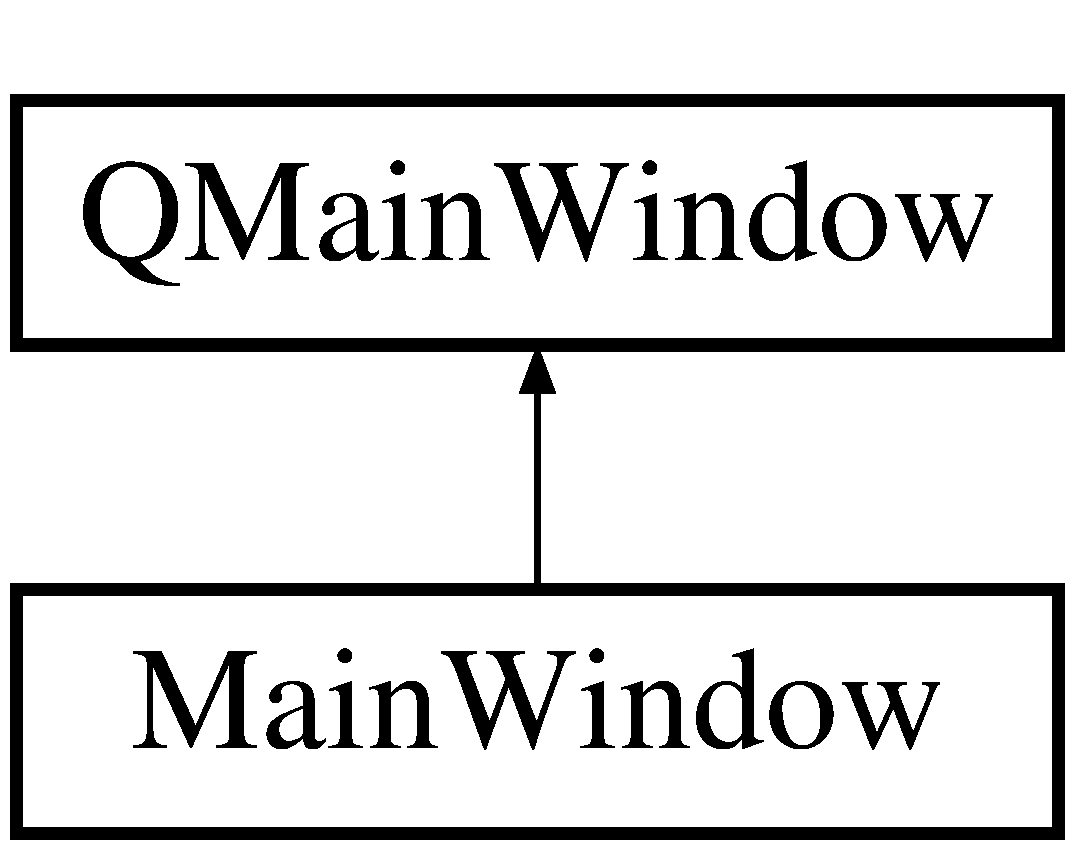
\includegraphics[height=2.000000cm]{classMainWindow}
\end{center}
\end{figure}
\subsection*{Public Member Functions}
\begin{DoxyCompactItemize}
\item 
\hypertarget{classMainWindow_a8b244be8b7b7db1b08de2a2acb9409db}{{\bfseries Main\-Window} (Q\-Widget $\ast$parent=0)}\label{classMainWindow_a8b244be8b7b7db1b08de2a2acb9409db}

\end{DoxyCompactItemize}


The documentation for this class was generated from the following files\-:\begin{DoxyCompactItemize}
\item 
mainwindow.\-h\item 
mainwindow.\-cpp\end{DoxyCompactItemize}

\hypertarget{classStereoVisionBlackBox}{\section{Stereo\-Vision\-Black\-Box Class Reference}
\label{classStereoVisionBlackBox}\index{Stereo\-Vision\-Black\-Box@{Stereo\-Vision\-Black\-Box}}
}
\subsection*{Public Member Functions}
\begin{DoxyCompactItemize}
\item 
\hypertarget{classStereoVisionBlackBox_ab157f91a5404792970d781ba9e2ad1b3}{{\bfseries Stereo\-Vision\-Black\-Box} (int rows, int cols)}\label{classStereoVisionBlackBox_ab157f91a5404792970d781ba9e2ad1b3}

\item 
bool \hyperlink{classStereoVisionBlackBox_adb780bea4a9c5594559d5e5575dc6c50}{add\-Calibration\-Images} (vector$<$ Mat $>$ left\-Imgs, vector$<$ Mat $>$ right\-Imgs)
\begin{DoxyCompactList}\small\item\em allows to add calibration images for left and right camera as vector lists. The images should be pairs showing exactly the same chessboard calibration pattern, altering the pose from pair to pair. Thus, the vector lists must have the same lenght. \end{DoxyCompactList}\end{DoxyCompactItemize}


\subsection{Member Function Documentation}
\hypertarget{classStereoVisionBlackBox_adb780bea4a9c5594559d5e5575dc6c50}{\index{Stereo\-Vision\-Black\-Box@{Stereo\-Vision\-Black\-Box}!add\-Calibration\-Images@{add\-Calibration\-Images}}
\index{add\-Calibration\-Images@{add\-Calibration\-Images}!StereoVisionBlackBox@{Stereo\-Vision\-Black\-Box}}
\subsubsection[{add\-Calibration\-Images}]{\setlength{\rightskip}{0pt plus 5cm}bool Stereo\-Vision\-Black\-Box\-::add\-Calibration\-Images (
\begin{DoxyParamCaption}
\item[{vector$<$ Mat $>$}]{left\-Imgs, }
\item[{vector$<$ Mat $>$}]{right\-Imgs}
\end{DoxyParamCaption}
)}}\label{classStereoVisionBlackBox_adb780bea4a9c5594559d5e5575dc6c50}


allows to add calibration images for left and right camera as vector lists. The images should be pairs showing exactly the same chessboard calibration pattern, altering the pose from pair to pair. Thus, the vector lists must have the same lenght. 


\begin{DoxyParams}{Parameters}
{\em left\-Imgs} & a vector containing the calibration images for the left camera. \\
\hline
{\em right\-Imgs} & a vector containing the calibration images for the right camera. \\
\hline
\end{DoxyParams}


The documentation for this class was generated from the following files\-:\begin{DoxyCompactItemize}
\item 
stereovisionblackbox.\-h\item 
stereovisionblackbox.\-cpp\end{DoxyCompactItemize}

%--- End generated contents ---

% Index
\newpage
\phantomsection
\addcontentsline{toc}{chapter}{Index}
\printindex

\end{document}
